\documentclass[sigconf,review,anonymous]{acmart}
%\documentclass[10pt, conference]{IEEEtran}

\usepackage[american]{babel}
\usepackage{booktabs}
\usepackage{caption}
\usepackage{color}
\usepackage{colortbl}
\usepackage{comment}
%\usepackage[keeplastbox]{flushend}
\usepackage{hyperref}
\usepackage{listings}
\usepackage{multirow}
\usepackage{soul}
\usepackage{tabularx}
\usepackage[textsize=scriptsize]{todonotes}
\usepackage{url}
\usepackage{xspace}
\usepackage{eurosym}
\usepackage{amsmath}
\usepackage{graphicx}
\usepackage{subcaption}

\usepackage{footnote}
\makesavenoteenv{tabular}
\makesavenoteenv{table}

\usepackage{array}

\newcommand{\captcha}{\textsc{captcha}\xspace}
\newcommand{\captchas}{\textsc{captcha}s\xspace}

\setcopyright{rightsretained}

\acmConference[ICSE'18]{International Conference on Software Engineering}{May 2018}{Gothenburg, Sweden} 
\acmYear{2018}
\copyrightyear{2018}

\begin{document}

\title{Can Today's Machine Learning Pass Image-based Turing Tests?}
%\title{Shooting Ourselves on the Foot:\\ How Today's Machine Learning Can Pass Image-Based Turing Tests}

\author{Apostolis Zarras}
%\orcid{1234-5678-9012}
\affiliation{%
  \institution{Technical University of Munich}
  \country{Germany}
}
\email{zarras@sec.in.tum.de}

\author{Ilias Gerostathopoulos}
\affiliation{%
  \institution{Technical University of Munich}
  \country{Germany}
}
\email{gerostat@in.tum.de}

\author{Daniel M\'endez Fern\'andez}
\affiliation{%
  \institution{Technical University of Munich}
  \country{Germany}
}
\email{daniel.mendez@tum.de}

\renewcommand{\shortauthors}{A. Zarras et al.}

%
% The code below should be generated by the tool at
% http://dl.acm.org/ccs.cfm
% Please copy and paste the code instead of the example below. 
%


\begin{abstract}
Artificial intelligence in general and machine learning (ML) in particular, although not new, have received much attention in recent years also thanks to current advancements in computational infrastructures. One prominent example application of ML is given by image recognition services that allow to recognize characteristics in images to classify them accordingly. One question that arises, also in light of current debates that are fueled with emotions rather than evidence, is to which extent such ML services can already pass image-based Turing Tests. That is, can ML services imitate human (cognitive and creative) tasks to an extent that their behavior remains indistinguishable from human behavior? If so, what does this mean from a security perspective?

In this paper, we report on a curiosity-driven study to critically evaluate a number of ML services by the degree to which they can be used to pass image-based Turing Tests. We do so by applying a number of publicly available ML services to 10.500 \captchas including approximately 100.000 images. Our results shall allow to critically reflect upon the implications of current advancements in AI in general, and in ML in particular.

\end{abstract}

\keywords{Machine learning, security, empirical study, We are awesome}

\maketitle


\section{Introduction}

Artificial Intelligence (AI) has been coined by pioneers like Alan Turing in the 1950's~\cite{turing1950computing} and deals ever since with the fundamental effort ``to automate intellectual tasks normally performed by humans'' \cite{deepLearning2017}. One core area of AI is machine learning (ML) where, in contrast to rather classical instruction-based programming where machines process given data sets based on predefined rules, machines are \emph{trained} with large data sets to recognize representation patterns in the data and produce the processing rules, thus, they ``learn'' how to recognize and classify given phenomena \cite{deepLearning2017}.

Thanks to recent advancements in computational infrastructures, machine learning itself, but also thanks to the availability of large data sets that are fundamental to ML, artificial intelligence has been making long and decisive strides forward from the 1990's on. These advancements are made along two main paths: $(i)$~the research in introducing new and improving existing ML techniques and methods (e.g., deep learning, convolutionary neural networks, Gaussian processes) and $(ii)$~the widespread adoption of ML techniques and methods in both research and practice. As for the latter, there exist nowadays many ``ML-as-a-service'' offerings, which simplify the access to and the use of powerful ML-enabled functionalities.  

A representative example of one such type of offering is given by image recognition services. A number of providers, from large companies such as Amazon, IBM, Google, and Microsoft, to startups such as Clarify and Cloudsight, offer paid services allowing other companies or individuals to add advanced image recognition capabilities to their systems. Such capabilities include, inter alia, classifying/labeling an arbitrary image with a number of tags at certain confidence levels, determining whether an image  contains a given element (object/person), or finding similar images in a collection.

Fueled by, at least from an application perspective, major advancements in machine learning, we can witness very optimistic marketing slogans accompanying available services (``build apps that see the world like you do''\footnote{\url{https://www.clarifai.com}}). Needless to say, also negative future scenarios on threats potentially imposed by ML are heavily spread in the public sphere\footnote{\url{https://www.nytimes.com/2017/07/15/opinion/sunday/please-prove-youre-not-a-robot.html}}. In fact, today's public debates are too often comparable to a hype
full of emotions and conventional wisdom rather than rational debates on basis of concrete evidence on the state of the practice and reasonable implications this has on security and safety issues. Without any prejudice and expectations on future applications of AI, one interesting and important question yet remains how far we have actually come as of today with current technologies. In other words, could current ML advancements pass the Turing Test, i.e., could they imitate human (cognitive and creative) tasks to an extent that their behavior remains indistinguishable from a human behavior?

\subsection{Problem Statement}

To the best of our knowledge, there exists little evidence about the extent to which Machine Learning currently can pass Turing Tests and the implications this has on topics like security. Indeed, there has been so far no systematic attempt to validate and compare the effectiveness and applicability of ML techniques in controlled settings. 

\subsection{Research Objectives}

With this paper, we contribute a curiosity-driven study with the aim to provide a first step in closing the knowledge gap on the state of ML with respect to (image-based) Turing Tests. That is, our goal is to critically evaluate a number of ML services by the degree to which they can be used to pass Turing Tests. This shall allow to critically reflect upon the implications current advancements in AI in general, and in ML in particular, have.

\subsection{Contributions}

Turing Tests are embodied in the latest versions of widely used \captcha services (e.g., Google's re\captcha). Image-based \captchas rely on the assumption that a specific task, in this case that of image recognition, is presumingly difficult for AI but easy for human beings based on their cognitive abilities and experiences. If the capabilities of currently available cloud-based ML services suffice to solve such problems, creating a automatic solver of image-based \captchas by relying on these services would be technically feasible and even economically viable. A consequent question therefore is for us: To which extent do image-based \captchas still pose a reliable Turing test and what are the security implications? Driven by this question, we make the following main contributions:

\begin{enumerate}
\item We investigate the effectiveness of in total \emph{six} image recognition ML services, and
\item we discuss the impact and implications on security.
\end{enumerate}

The reason behind choosing image-based \captchas as our benchmark is manifold. First, they provide a neutral ground for comparing the different image recognition services, as none of these services is tailored to breaking \captchas, i.e. to pass the Turing Test based on image recognition. A further reason is of pragmatic nature: \captchas are, same as ML services, largely available to the public facilitating studies, replications, and the public discourse.
Finally, we consider it important that the demonstration facilitates a discussion on a larger scale since it shall put forward important security considerations for the future of ML in general, but also of \captchas in particular. We consider a re-evaluation of mechanisms such as ones incorporated in the de-facto standard \captchas to be important, because of their criticality to the security of today's systems.

\subsection{Outline}

The remainder of this paper is structured as follows. In Sect.~\ref{sec:RelWork}, we discuss fundamentals and work related to our contribution. In Sect.~\ref{sec:StudyDesign} we introduce our study design before summarizing the results in Sect.~\ref{sec:StudyResults}. In Sect.~\ref{sec:ImpactImplications} we discuss the impact and implications of our results before finally concluding our paper with a summary of conclusions and an outline of future work.


\section{Fundamentals and Related Work}
\label{sec:RelWork}

\subsection{Image Recognition via Machine Learning}

\subsection{Image Recognition Services}



\subsection{CAPTCHA}

\todo[inline]{What is a captcha.
Origins.
text-based. problems with text-based. 
image-based. 
popular services now (recaptcha, facebook captcha).}

The term \captcha (i.e., \emph{Completely Automated Public Turing Test To Tell Computers and Humans Apart}) was first introduced by von Ahn et al.~\cite{von2003captcha} in an attempt to create automated tests that only humans could pass.

what are the current capabilities 

\subsection{Related Work} 

The suitability of \captchas as a means to implement Turing Tests in a usable manner has been discussed for some years now. In particular, Bursztein et al.~\cite{bursztein2014end} report on a joint collaboration from 2014 between Standford university and Google where they already explored techniques to break \captchas. \todo{https://www.usenix.org/system/files/conference/woot14/woot14-bursztein.pdf} In fact, their results indicated already to the insecurity of purely text-based \captchas, thus, strengthening the confidence in the need to foster image-based \captchas. Besides further work investigating the limitations of text-based \captchas~\cite{starostenko_breaking_2015,baecher_breaking_2011,cruz-perez_breaking_2012}, but also audio-based \captchas (see, e.g. the work by Kopp et al.~\cite{kopp2016mimic}), much of research effort has since then concentrated on follow-up investigations of image-based \captchas.

There are reports on successfully breaking the \captcha challenge, i.e. image-based Turing Tests, such as the one by Goodfellow et al,~\cite{goodfellow2013multi}. Here, the authors \todo{Check: https://arxiv.org/pdf/1312.6082.pdf}

Follow-up work, such as the one by Osadchy et al.~\cite{osadchy2017no}, propose mechanisms to distort images in order to make breaking corresponding \captchas automatically more difficult. 

\todo{seems also quite related as they propose mechanisms to distort images so that current deep learning based techniques should not be able to break. See also https://eprint.iacr.org/2016/336.pdf}

%Googles revised reCaptch challenge now in scope of more recent work:
The latest work, to the best of our knowledge, attempting to break the current version of Google's \captchas is reported by Sivakorn et al.~\cite{sivakorn2016robot}. The authors propose an attack that makes use of deep learning technologies to annotate images. They focus, same as we do, on trying to automatically break reCaptcha challenges and and succeed in roughly 70\% of the cases. Although the scope of their work differs in the sense of providing an (also technical) analysis of \captchas, their work inspired some technicalities of our own study design to provide a broader analysis of publicly available ML services. In particular, \todo{summarise least common denominators as the data they stored for the images... end with explanation where we differ} 



\todo[inline]{Further work: Learning to Associate Words and Images Using a Large-scale Graph (https://arxiv.org/abs/1705.07768)}

\section{Study Design}
\label{sec:StudyDesign}

Our overall objective is to better understand the extent to which image-based \captchas still pose a reliable Turing test and what the implications are on security. To this end, we formulate a set of research questions described below before introducing the data collection and analysis procedures. We will conclude with an outline of the validity procedures taken to mitigate the major threats to the validity in advance.

\subsection{Research Questions}
To achieve our overall objective, we first need to understand what the potential of ML is with respect to image-based \captchas and accordingly design our study along three research questions:
\begin{itemize}
\item[\textbf{RQ~1}] What is the precision and recall of ML Services?
\item[\textbf{RQ~2}] What is the absolute accuracy of ML services to break \captchas? 
\item[\textbf{RQ~3}] What is their sufficient accuracy of ML services to break \captchas? 
\end{itemize}

First, we want to understand what the precision and recall is of given ML services to recognize the images included in the \captchas. This allows us getting a basic understanding on the general potential of the services. As the images strongly differ in the content they represent (e.g. a river versus a car), we want to further understand whether there are differences with respect to the particularities of the images themselves and what they represent respectively. Once we understand the general potential of the ML services, we want to analyze the extent to which they can be used to ``break'' \captchas (containing sets of images of same and different categories), i.e., how well available services can be trained to bypass the today's wide-spread image-based Turing tests.

We do so in two steps (RQ~2 and 3): First, by analyzing the \emph{absolute accuracy} of the services in terms of their potential to correctly categorize all images of single \captchas into labels frequently used. Second, image-based \captchas, if used in context of security mechanisms such as login mechanisms, usually allow for a specific failure tolerance (e.g. by allowing to classify on image wrongly). To lay the ground for our second contribution discussing the impact on security issues, we want to know what their \emph{sufficient accuracy} is to break \captchas. 

Based on this overall analysis, we conclude with a discussion of the impact and the implications on security issues (our second contribution). Given that this discussion is based, in parts, on analytical work, we also provide a brief discussion of the security impact analysis procedure to the extent necessary to reproduce our work. This discussion can be found in Sect.~\ref{sec:ImpactImplications}.

\subsection{Data Collection and Analysis}
In the following, we introduce the data collection and the analysis procedures.

\subsubsection{Data Collection}

The raw dataset of our study consists of the images contained in 10,500 image \captchas. %Each image is annotated with a boolean value indicating whether it is a correct answer to the \captcha challenge and with the results of six image recognition services. 
For our study we further used the 6 image-recognition services listed in Tab.~\ref{services-table}. To conduct our study where we compared these image-recognition services, we had to first prepare the data by establishing an oracle (ground truth) which we used to train the ML services. Afterwards, we employed the services and analyzed the results with respect to our research questions.

In brief, to prepare the dataset for our study, we 
\begin{enumerate}
\item retrieved the images contained in the 10500 \captchas (about 100.000 images),
\item manually solved them in a pair of researchers in the sense of annotating labels to the \captchas\footnote{Here, the first two authors solved the \captchas.}, and finally
\item submitted each image to the image recognition services, retrieved, and stored the results.
\end{enumerate}
The last step considers both the training phase of the ML services and the actual study which we call the test phase. See also Sect.~\ref{sec:TestingAndTraining} for further information.

In the following, we provide details for each of the aforementioned steps.

First, we leveraged Google's re\captcha service\footnote{\url{https://developers.google.com/recaptcha}} automatically via a JavaScript to create our corpus of image \captchas. For ethical reasons and to not interfere with a legitimate website traffic, we set up re\captcha on a website created for the sole purpose of our study. We then scraped the contents of the re\captcha challenges; we repeated the process 10,500 times. To (semi-)automate the process, we utilized \emph{Selenium}, a software-testing framework for web applications that has the ability to programatically control a real web browser, in our case Google Chrome. During each challenge, we scraped and saved in a MongoDB database a document containing the category of the challenge, (e.g., ``Select all images with street numbers'') and the individual images, both their Binary representation and the MD5 hash of them. Since re\captcha returns a single image file and the image grid (e.g., ``3x3''), we cropped the larger image according to the grid to obtain the individual images. Such an exemplary image can be taken from Fig.~\ref{image-example}.

Second, we went through all collected 10,500 challenges and manually solved them by marking the images that were correct answers to each challenge with a \texttt{true} flag. The effort for the manual task was approximately 70 person hours. It is worth mentioning here that not all the images have an unambiguous semantics (e.g. a building can have also a store). Hence, in cases were the actual semantics of an image is not completely clear, we directly discussed them between the pair of researchers.

\begin{figure}[t]
\centering
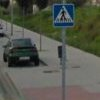
\includegraphics[width=0.5\columnwidth]{images/car.jpg}
\caption{An exemplary image that was marked as correct answer to the challenge of category ``Select all images with cars.''}
\label{image-example}
% find it in MongoDB Compass with: 
% {"_id":{"$oid":"592c072fe922892c37ac8712"}}
\end{figure}

\begin{table}[t]
\centering
\caption{Services used in the study. The example results correspond to the image of Figure~\ref{image-example}.}
\label{services-table}
\begin{tabularx}{\columnwidth}{p{5em}p{5.5em}X}
\toprule
\textbf{Service}              & \textbf{Endpoint} & \textbf{Example Result (Relevant Fragments)} \\
\midrule
\multirow{6}{*}{\shortstack[l]{Google\\ Cloud Vision}} & \multirow{6}{*}{detect\_labels} &
\qquad 0: ``mode~of~transport''\\
&& \qquad 1: 0.8423645;\\
&& \qquad 0: ``lighting''\\
&& \qquad 1: 0.63189656;\\
&& \qquad 0: ``signage''\\
&& \qquad 1: 0.6097285; ...\\
\midrule
\multirow{6}{*}{\shortstack[l]{IBM Watson\\ Visual\\ Recognition}} & \multirow{6}{*}{classify} & classes:\\
&& \qquad class: ``intersection''\\
&& \qquad score: 0.735;\\
&& \qquad class: ``junction''\\
&& \qquad score: 0.799;\\
&& \qquad class: ``highway''\\
&& \qquad score: 0.58; ...\\
\midrule
\multirow{7}{*}{\shortstack[l]{Amazon\\ Rekognition}} & \multirow{7}{*}{detect\_labels} & Labels:\\
&& \qquad Name: ``Automobile''\\
&& \qquad Confidence: 58.2802352;\\
&& \qquad Name: ``Car''\\
&& \qquad Confidence: 58.2802352;\\
&& \qquad Name: ``Vehicle''\\
&& \qquad Confidence: 58.2802352 \\
\midrule
\multirow{7}{*}{\shortstack[l]{Microsoft\\Computer\\ Vision}} & \multirow{7}{*}{describe} &
captions:\\
&& \qquad text: ``a~sign~on~the~side~of~a~road''\\
&& \qquad confidence: 0.9499872;\\
&& tags: \\
&& \qquad 0: ``outdoor''; \\
&& \qquad 1: ``street''; \\
&& \qquad 2: ``grass''; ... \\
% Microsoft\newline Computer Vision & 
% describe &  
% $captions: $\newline
% $~~text:$\newline $~~~~``a~sign~on~the~side~of~a~road"$\newline
% $~~confidence: 0.9499872$
% $tags: $\newline
% $~~0:``outdoor";$\newline 
% $~~1:``street";$\newline 
% $~~2:``grass";~...$\\
\midrule
\multirow{7}{*}{\shortstack[l]{Clarify\\ Visual Search}} & 
\multirow{7}{*}{predict} & concepts: \\
&& \qquad name: ``road''\\
&& \qquad value: 0.9973230;\\
&& \qquad name: ``street''\\
&& \qquad value: 0.9972282;\\
&& \qquad name: ``car''\\
&& \qquad value: 0.991663; ...\\
\midrule
Cloudsight & 
image\_request & name: ``Pedestrian~signboard''\\
\bottomrule
\end{tabularx}
\end{table}

Third, we applied the image-recognition services to automatically label each of the collected images with metadata describing the image. To this end, we leveraged the image labeling APIs of our six different image recognition services we evaluated. Each API required a jpeg-encoded file as input and provided a JSON-encoded response with metadata in the form of labels, concepts, classes, tags, or captions. For the remainder of the paper, we refer to these as \emph{keywords}. With the exception of Cloudsight, all services provided a numeric value capturing the confidence value or score of each keyword, to which we refer from now on as \emph{confidence}. An overview of the service names, their API endpoints for image labeling, and their exemplary results is depicted in Table~\ref{services-table}. 
We accessed all services through Python clients and saved the obtained raw results directly in the database for later analysis.
%\todo{Explain table columns}

Finally, in context of the data collection, we needed to issue approximately 100,000 requests per service. As this exceeded the evaluation quota per service, we opted, 
where necessary and possible for specific (academic) licenses.

\subsubsection{Testing and Training Data}
\label{sec:TestingAndTraining}

To obtain the results described in the next section, we split the collected data, i.e. our corpus of 10.500 image \captchas, into two disjunct sets: a training set and a testing set. The first is used to train the ML services, the last to run the actual study where we evaluate the ML services. That is, while the training set is used to create the meta-classifiers as described below, the testing set is used for evaluating the accuracy of the ML services in solving \captcha challenges in the following way (RQ 1 to 3). 

The training set constitutes a randomly sampled (yet equally distributed along the different categories) 90\% of the collected images; the testing set constitutes the remaining 10\% of the images.

%Given a challenge of category $C$, we tried to solve it by looking at the results retrieved from a service $S$ for each of the images contained in the challenge.  We marked as \texttt{true} the images whose responses from $S$ $(i)$~contained at least one of the optimal keywords of the [$S$,$C$] pair and $(ii)$~the accompanying confidence was greater or equal to the confidence threshold of the matching optimal keyword.
%In other words, we used the meta-classifiers created via analyzing the training set in order to solve the challenges of the testing set as accurately as possible.


\subsubsection{Data Analysis}
To answer RQ~1, we calculate the precision and recall based and used the manually classified images as a reference to the ground truth.

To answer the research questions 2 and 3, we needed to calculate the accuracy of the ML services with respect to break the \captchas. To this end, we devised a method to compare the results of each service with the ground truth of previously manually labeled images. One key challenge was to build a meta-classifier that predicts, based on the results of a service, whether each individual image is a correct answer to its encompassing challenge or not. We built such a meta-classifier for each service $S$ and for each challenge category $C$. We built each meta-classifier for [$S$, $C$] following three main steps: $(i)$~Collect all keywords $K$ retrieved from $S$ for images belonging to the challenges of $C$; $(ii)$~For each keyword, find the confidence threshold $T$ that yields the highest accuracy in predicting a correct (\texttt{true}/\texttt{false}) flag for an image; $(iii)$~Find the best combination of [$K$, $T$] pairs with the highest accuracy in predicting an accurate answer for a challenge.

At first, we collected all the keywords that were retrieved from $S$ for all the images that belonged to a challenge of category $C$. This was straightforward in all the services except for Microsoft's, whose response contains both a text with a confidence, and a number of tags (see Table~\ref{services-table}). We chose to extract the keywords for this service by tokenizing the text and omitting the tags. 

Next, for each keyword \textit{K}, we assumed a confidence threshold \textit{T}. We went through all images of $C$ and corresponding responses from $S$ and marked as true positive the cases where the image was manually labeled as correct answer to the challenge and $(i)$~$K$ was found by String matching (after converting all Strings to lowercase) in the response of $S$ and $(ii)$~the retrieved confidence was equal or higher to $T$. Accordingly, we calculated the number of true negatives, false positives, false negatives. Based on the confusion matrix, we also calculated the per-case \textit{accuracy} by diving the sum of true positives and true negatives to the total number of images. 
Technically, we started with a threshold value of $0$ and increased it with a step of $1$ up to $100$. We applied the above process for each $K$ in the [$S$, $C$] pair. An example of the produced data set is depicted in Table~\ref{extracted-thresholds-example}. As can be seen, with increasing confidence thresholds values, accuracies decrease since the comparison becomes stricter. Having this data set in place for each K, selecting the ``best'' confidence threshold was simply a matter of picking the one with the highest accuracy. 

In case two or more thresholds had the same accuracy (e.g., 48--50 in Table~\ref{extracted-thresholds-example}), we selected the one with the highest value to avoid potential false positives.

Finally, we created a list of all the keywords along with their best confidence thresholds and the accuracies that correspond to these thresholds; we sorted the list by the accuracies. For instance, for the [AWS, ``Select all images with cars''] case, the following list was created (showing only the first 5 elements):

\begin{lstlisting}[caption={Some Java code},label={lst:label},language=Java]
// Code...
\end{lstlisting}

\begin{lstlisting}[caption={Some Java code},label={lst:keywords},]
[automobile, 50, 75.46%],
[car, 50, 75.79%],
[vehicle, 50, 75.10%],
[highway, 56, 63.41%],
[freeway, 56, 63.05%],
...
\end{lstlisting}

As the example shows, trying to find the keyword ``automobile'', accompanied by a confidence greater or equal to 50\%, in the response of the AWS service to an image of a ``cars'' challenge is a promising way of getting an accurate prediction on whether to select this image as an answer or not. However, will the prediction improve if we include more [$K$, $T$] pairs? If so, what is the optimal number of pairs that should be included? 

To investigate these questions, we calculated the number of challenges that would be accurately solved (without any mistake) when considering only the head of list. Specifically, we marked as \texttt{true} the images whose responses from $S$ $(i)$~contained the keyword of the head of the list and $(ii)$~the accompanying confidence was greater or equal to the confidence threshold of the head of the list. In our example, this case is when the response of the AWS service for images belonging to the ``cars'' category contains the keyword ``automobile'' with a confidence greater or equal to 50\%. We then compared the marked images to the manually labeled ones---a match indicated an accurate solution of the challenge.

%\todo{Please explain the abbreviations in the table}
\begin{table}[t]
\centering
\caption{Excerpt from generated data set for the keyword ``automobile'' for the the AWS service and for the ``Select all images with cars.'' challenge category. TP stands for true positives, TN for true negatives, FP for false positives, FN for false negatives.}
\label{extracted-thresholds-example}
\begin{tabular}{cccccc}
\toprule
\multicolumn{1}{c}{\centering \textbf{Threshold}} & 
\multicolumn{4}{c}{\centering \textbf{Confusion Matrix}} &
\multicolumn{1}{c}{\centering \textbf{Accuracy (\%)}}
\\
\cmidrule(lr){2-5}
 & \textbf{TP}& \textbf{TN}  & \textbf{FP} & \textbf{FN} & 
 %(TP+TN/TP+TN+FP+FN)
 \\ 
\midrule
48 & 465 & 1627 & 3  & 677 & 75.46 \\ 
49 & 465 & 1627 & 3  & 677 & 75.46 \\ 
\rowcolor{lightgray} 50 & 465 & 1627 & 3  & 677 & 75.46 \\ 
51 & 462 & 1627 & 3  & 680 & 75.36 \\ 
52 & 457 & 1627 & 3  & 685 & 75.18 \\ 
53 & 451 & 1627 & 3  & 691 & 74.96 \\ 
\bottomrule
\end{tabular}
\end{table}

We repeated the above process by considering the first two items in the list, then the first three, and so on. In the end, we were able to determine the [$K$, $T$] pairs that can yield the most accurate predictions---we call these pairs ``optimal keywords'' for the [$S$,$C$] pair. In our example, these correspond to the first four items of \todo{list (1)}. From a practical perspective, this means that considering also the fifth item or any more items should not yield an increase in the accuracy of the predictions. 

\section{Study Results}
\label{sec:StudyResults}

In this section, we present the results of our study and structure them according to the research questions. For each question, we first report on the results and then provide a preliminary (subjective) interpretation.

\subsection{Population}

\begin{figure}[t]
\centering
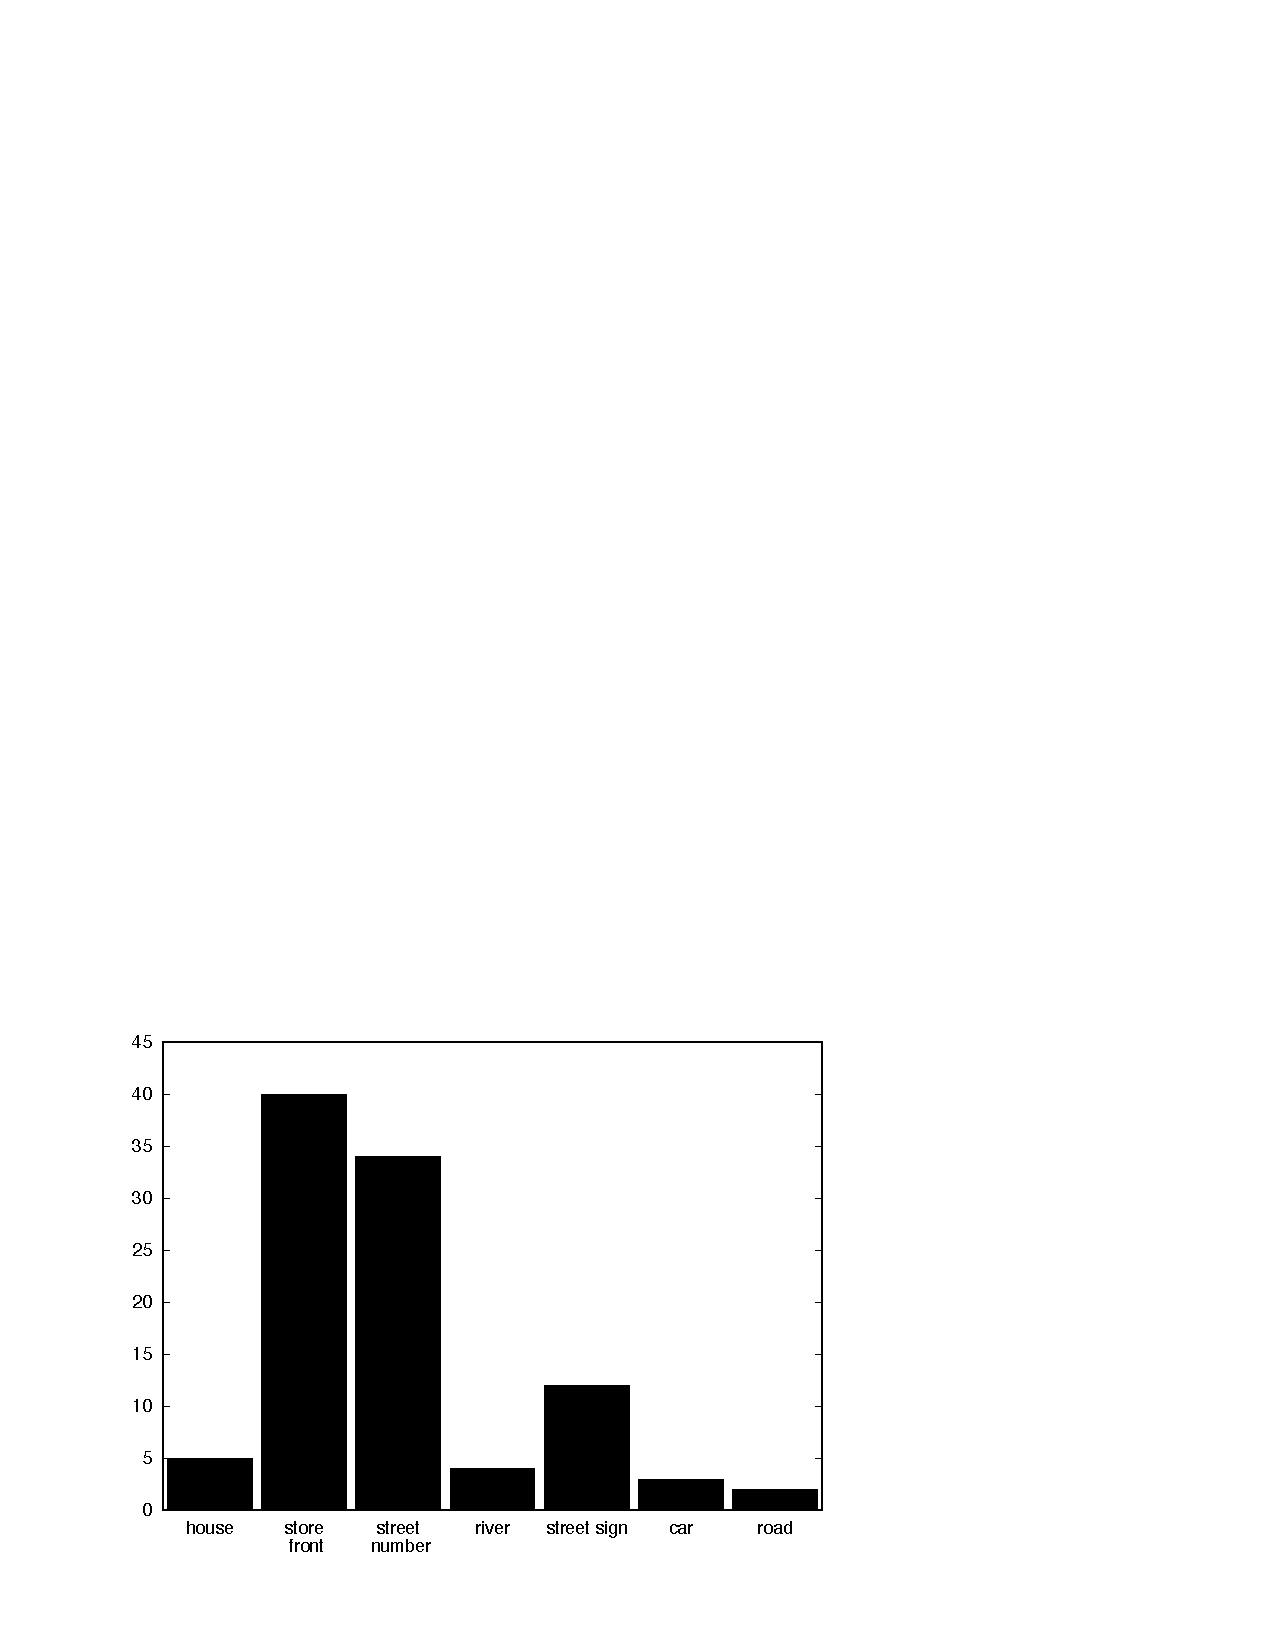
\includegraphics[width=\columnwidth]{images/captcha-distribution.pdf}
\caption{Distribution (in percentage) of collected \captchas in categories.}
\label{res-captcha-distribution}
\end{figure}

Our corpus consists of 10,500 \captchas belonging to seven different categories. 
Each category corresponds to the original prompt of the challenge such as, ``Select all images with house/store front/street number''. 
The distribution of \captchas per categories is depicted in Figure~\ref{res-captcha-distribution}.
As can be seen, the two most popular categories are \texttt{store~front} and $street~number$, which occupy 40\% and 34\% of the study data, respectively.
The smallest category, $road$, amounts to 2\% of the study data, in particular to 192 \captchas.
Each \captcha contained 8, 9 or 16 images (\captcha \textit{size}) arranged in a grid of 2x4, 3x3 and 4x4, respectively. 
\captchas of different sizes were not uniformly distributed in the categories. 
Instead, 16-sized \captchas belonged exclusively to the $street~sign$ category, 8-sized ones belonged exclusively to the $store~front$ category, 
and 9-sized ones belonged exclusively to the one of the other five categories. 
We discuss how the different per-category sizes may have influenced the results of our study in the next sections\footnote{We could have normalized the results by artificially enforcing size 8 for all categories, however we chose to preserve the original \captcha sizes in order to be able to draw valid conclusions on the ability to break the original \captchas.}.
%The average number of images per \captcha was 9.44; therefore, the total number of images that we processed was 99,108 (approx. $9.44*10,500$). 

The total number of images we milked/harvested/collected and processed was 99,108 (approximately 9.44 images per \captcha).

\subsection{RQ~1: Precision and Recall of ML Services}

\begin{figure}[t]
\centering
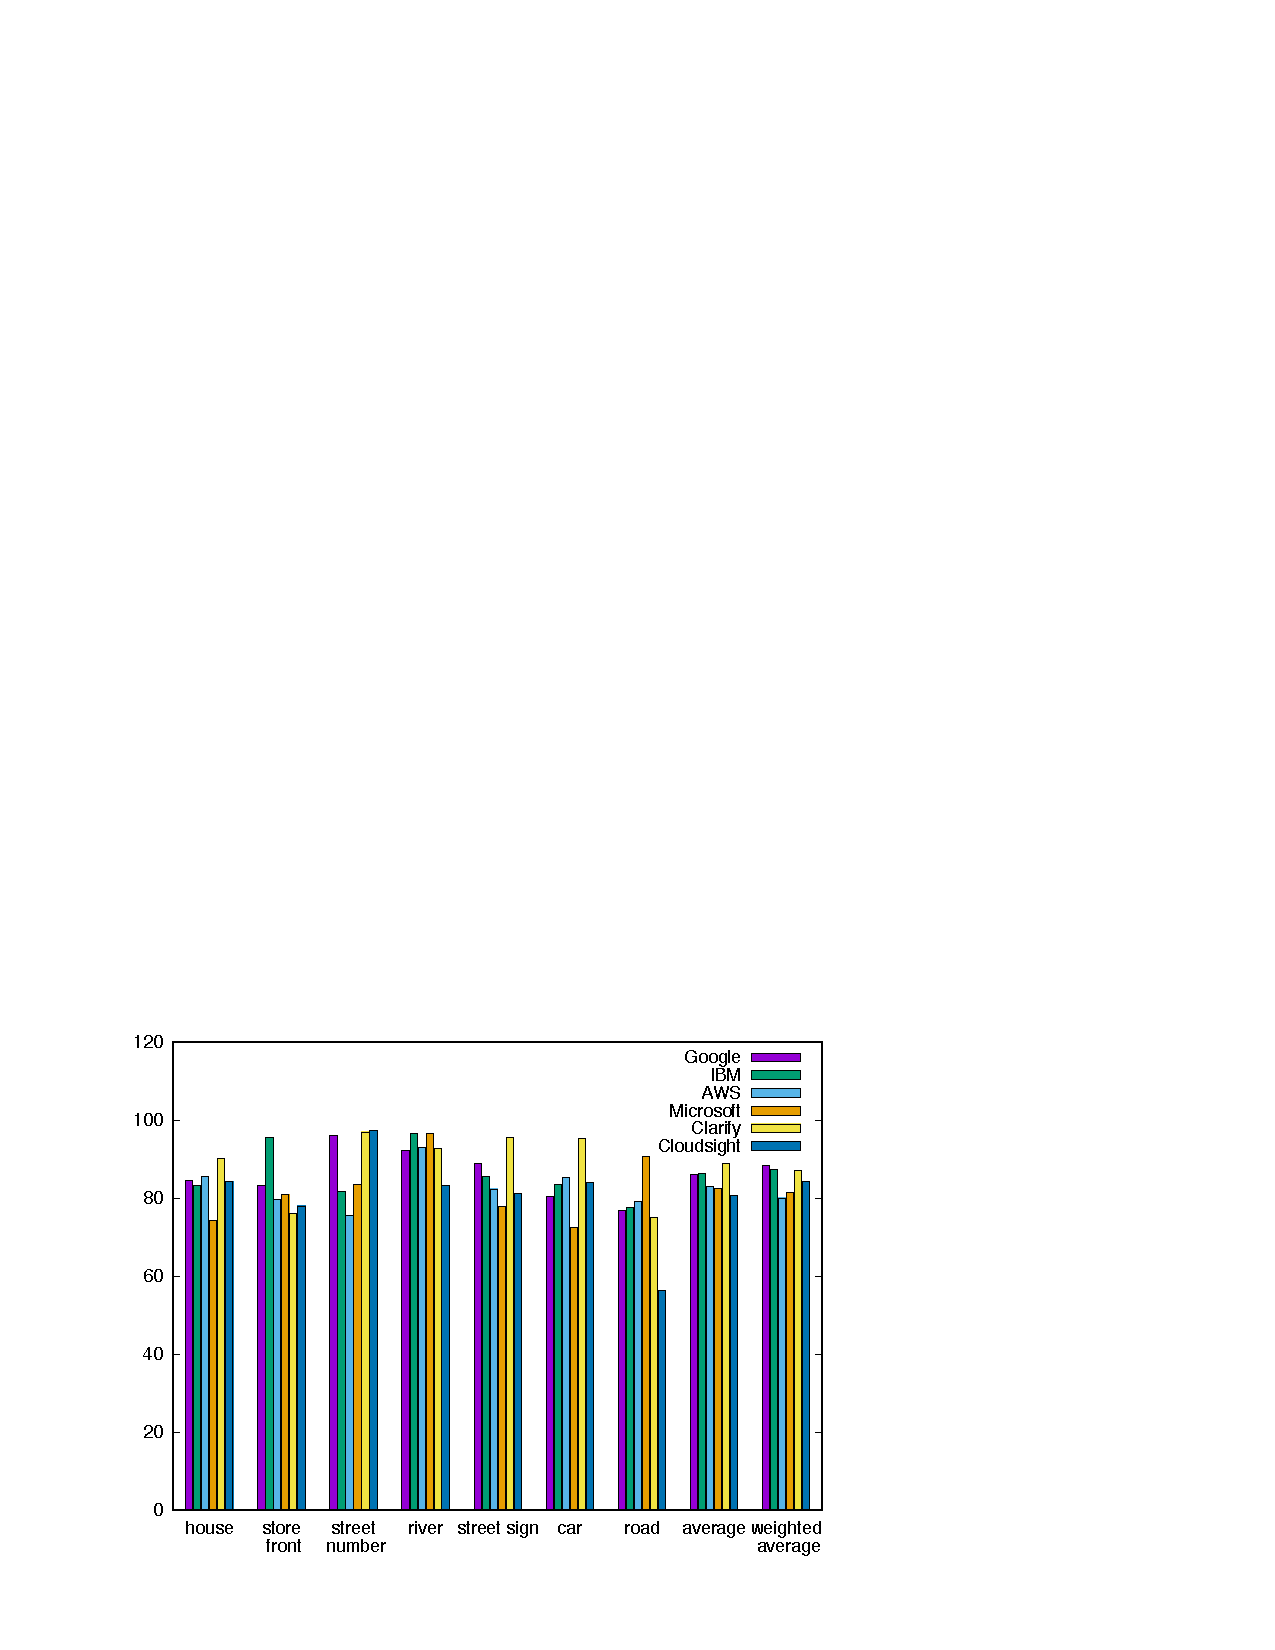
\includegraphics[width=\columnwidth]{images/precisions-1.pdf}
\caption{Precision of ML services in classifying an image as a correct answer to the encompassing \captcha challenge.}
\label{res-precisions}
\end{figure}

\begin{figure}[t]
\centering
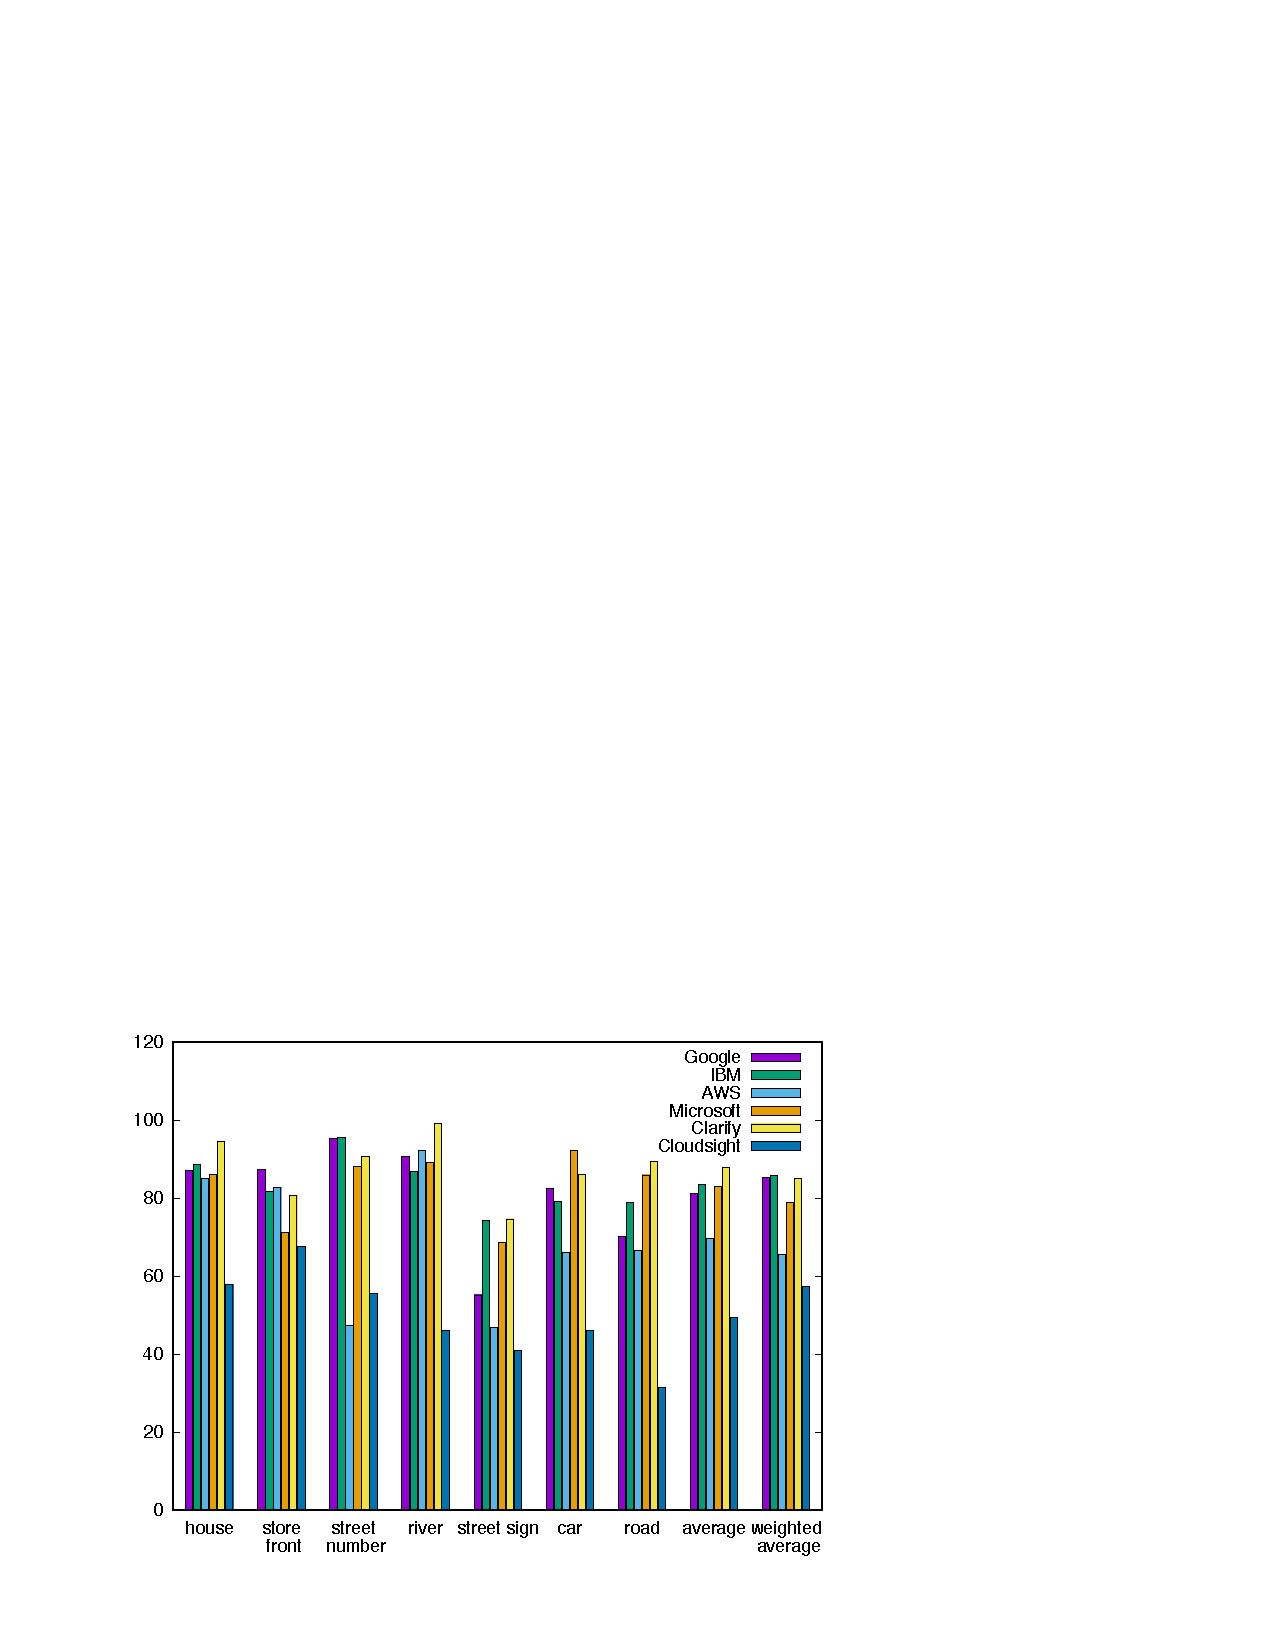
\includegraphics[width=\columnwidth]{images/recalls-1.pdf}
\caption{Recall of ML services in classifying an image as a correct answer to the encompassing \captcha challenge.}
\label{res-recalls}
\end{figure}

To investigate the differences between the performance of ML services in the different categories, we calculated the precision and recall of our meta-classifier that corresponds to a service-category pair across all images contained in all \captchas of the category. The results are depicted in Figures~\ref{res-precisions} and~\ref{res-recalls}. 

A first observation from Figure~\ref{res-precisions} is that, with a single exception that of $Cloudsight$ in $road$, all services score precision higher than 70\% in all categories, while in five categories the best precision is 95\% or higher. On average, the best precision (irrespective of the service providing it) is 94\%. 

When looking at the results of the services across all categories (two rightmost groups in the Figure~\ref{res-precisions}), $average$ is the mean value of calculated per-category precisions, while $weighted~average$ is the precision calculated on the total number of images, irrespective of the category of their encompassing \captchas.  Both statistics yield values between 81\% and 87\%, with small variations between the services.

Figure~\ref{res-recalls} depicts the recalls of our meta-classifiers corresponding to each category-service pair. 
The best recall per category ranges from 75\% to 99\% with an average value of 90\%. The categories with the highest recalls are $house$, $street~number$, and $river$, while the one with the lowest recalls is $street~sign$.
With respect to the services, $Cloudsight$ scores consistently low in all categories (an average of 49\%). The rest of the services score consistently high (more than 80\% on average), with the exception of $AWS$ which scores a mere 47\% in both $street~number$ and $street~sign$ (and obtains an average recall of 70\%).

\subsubsection*{Interpretation}
Looking at both the results of precision and recall analysis and the absolute and sufficient accuracy analysis, we can make the following interpretations regarding the performance of the services. 
First, for the two services that score low in accuracy, $AWS$ and $Cloudsight$, this is due to low recall of the respective meta-classifiers. 
This is illustrated by the case <$AWS$, $street~number$> in which the sufficient accuracy is 24\% (Figure~\ref{res-broken-captchas}) and the corresponding recall is 47\%.
It is also shown in the case of $Cloudsight$, which scores high in accuracy but low in recall, a result that explains the low accuracies values.

\todo{Key TAKEAWAYS?}






\subsection{RQ~2: Absolute Accuracy of ML Services}

\begin{figure}[t]
\centering
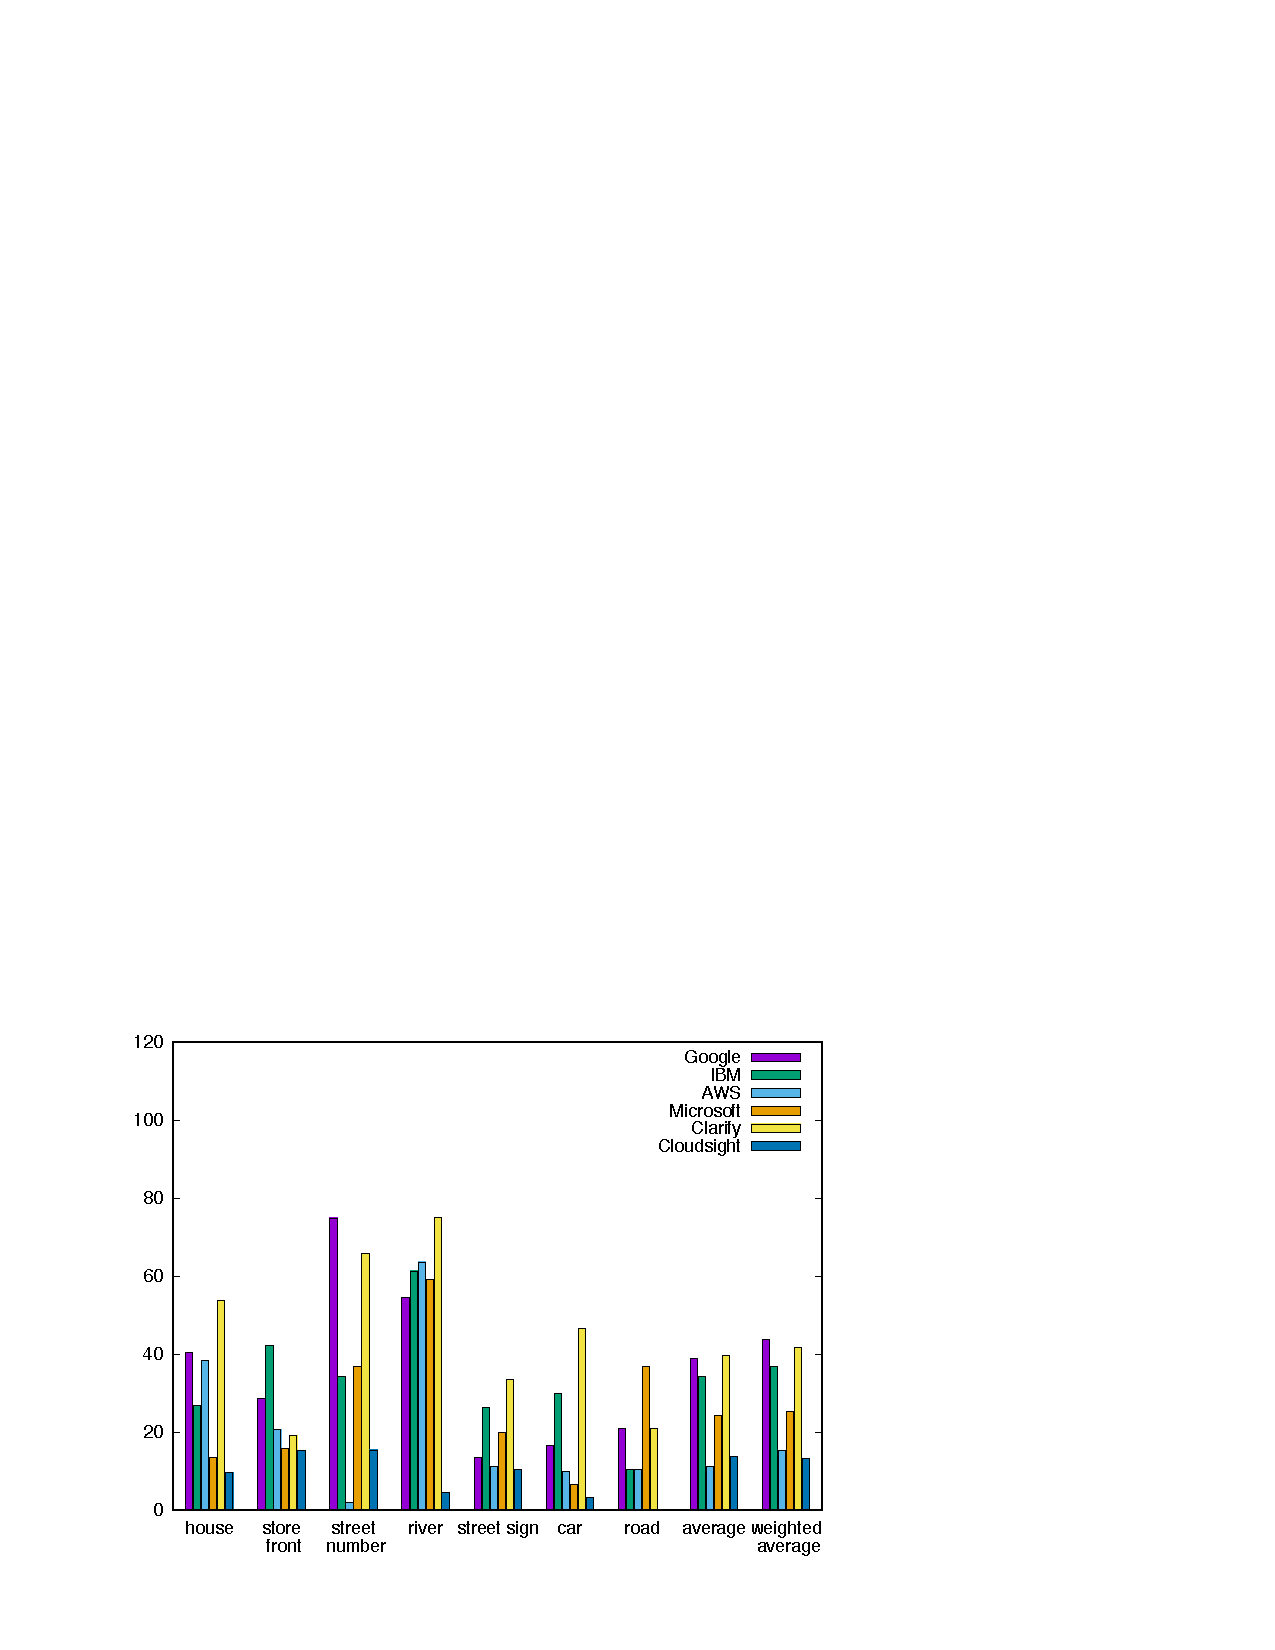
\includegraphics[width=\columnwidth]{images/accuracies-1.pdf}
\caption{Absolute accuracy (in percentage) of ML services: solving CAPTCHAs without tolerating any mistake.}
\label{res-accuracies}
\end{figure}

Figure~\ref{res-accuracies} depicts the results for the absolute accuracy case, that is, when trying to solve \captchas without tolerating a single mistake in the binary classification (\textit{selected} or \textit{not selected}) of the images included in each \captcha.

The results are grouped according to each of the 7 categories.
The second group from the right, $average$, is the mean value of calculated per-category accuracies. 
Finally, the rightmost group, $weighted~average$, is the accuracy calculated on the total number of \captchas, irrespective of their category. Since some categories contain more \captchas, these two values are different for each service, with the weighted average ``boosting'' the services which score higher in the popular categories of $street~number$ and $store~front$.

The results indicate that for each category there is at least one service that scores higher than 35\%, with two categories, $street~number$ and $river$, having services that score up to 75\%.
Overall, the services score lower in $store~front$ and $street~sign$ and higher in $river$. 
There are also many differences in the performance of the services in different categories.
For example, $Microsoft$ and of $Google$ are the most accurate services in $road$ and $street~number$, respectively, while $Clarifai$ is the most accurate in $house$, $river$, $street~sign$, and $car$. 
$AWS$ scores high in $house$ and $river$, but extremely low (2\%) in $street~sign$. 
At any rate, on average, the $Clarifai$ and $Google$, closely followed by $IBM$, are the most accurate services, with an average accuracy of close to 40\%.
\todo{Add precision and recall here?}

\subsubsection*{Interpretation}
With the exception of $Clarifai$, resp. $Cloudsight$, which is scoring consistently high, resp. low, the high variation in the results of the other services can be attributed to the difference in the datasets used in the training of their internal ML classifiers. 

The reason why some categories yield lower accuracies seems more clear. 
A street number, although blurry, is entirely contained in an image; a river can be recognized by its characteristic shape and color.  
A street sign, on the contrary, does not have any characteristic color and its characteristic shape is often not identifiable as it is typically not entirely contained in an image. Human cognition should be able to easily identify fragments of street signs by imagining the missing parts; it seems that this is challenging for ML algorithms.

Finally, although the average accuracy of services is not high, please note that the absolute accuracy test is also challenging for humans. That might be also the reason why \captcha services such as re\captcha typically allow for one mistake per challenge. In the following, we report our results for this very case.

\todo{Key TAKEAWAYS}

\subsection{RQ~3: Sufficient Accuracy of ML Services}

\begin{figure}[t]
\centering
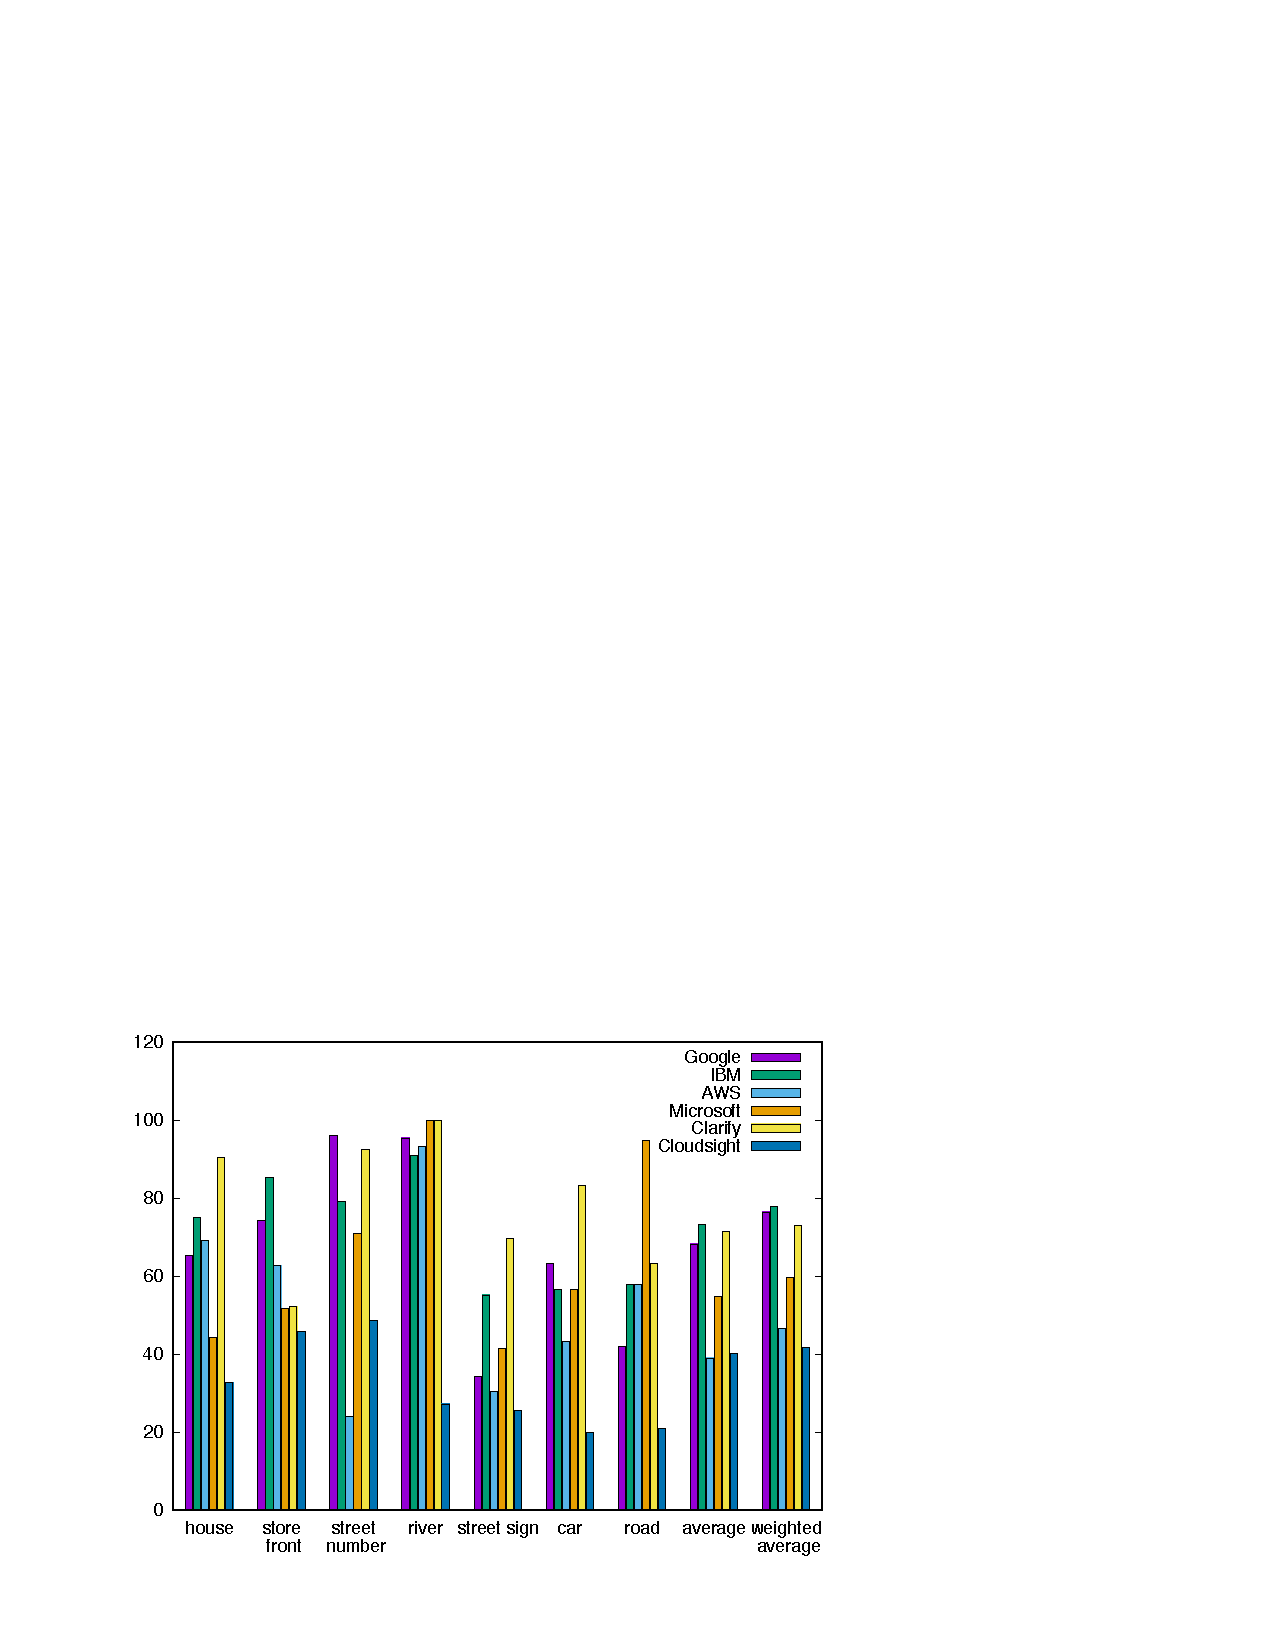
\includegraphics[width=\columnwidth]{images/broken-1.pdf}
\caption{Sufficient accuracy (in percentage) of ML services: solving CAPTCHAs by tolerating one mistake.}
\label{res-broken-captchas}
\end{figure}

Figure~\ref{res-broken-captchas} shows the results for the sufficient accuracy case, that is, when trying to solve \captchas by tolerating one mistake in the binary classification of images included in each \captcha. 

A first observation is that for each category there is at least one service with sufficient accuracy 70\% or more; for three categories, the best accuracy is even 95\% or more ($river$, $street~number$, $road$).
On average, the best accuracy (irrespective of the service providing it) is 88\%.
Similarly to the absolute accuracy case, the $street~sign$ is the worst performing category overall. We can also observe sharp differences in the performance of services in some categories: $AWS$ scores a mere 24\% in $street~number$, where the service of $Cloudsight$ seems the second most inaccurate with close to 50\%. All other services score more than 70\%.
In the categories $house$ and $road$, the services of $Clarifai$ and of $Microsoft$ stand out as far better than the other services scoring accuracies of 90\% and 95\%, respectively.

The two rightmost groups have been calculated as it was the case for the absolute accuracy. It seems clear that, on average, the three most accurate services are the ones offered by $IBM$, $Clarifai$, and $Google$ with a weighted average accuracy 78\%, 76\%, and 73\% respectively.
$Microsoft$ scores a weighted average accuracy of 60\%, while $AWS$ and $Cloudsight$ score 47\% and 42\%, respectively. 

Finally, comparing the results of the sufficient accuracy case with the absolute accuracy, we can observe that in most categories the relative difference between the services accuracies is preserved, while the absolute values have strongly increased. When looking at the best performing services per category, their precision across the two cases is increased on average by 36 percentage units, with a minimum increase of 21 units ($Google$ for $street~number$) and a maximum of 58 units ($Microsoft$ for $road$).  

\subsubsection*{Interpretation}
Similarly to the absolute accuracy case, the sharp variations in the performance of services across different categories can be explained by different datasets used in the training of the internal ML classifiers.
\todo{Can we add something else here? or shall we merge this interpretation with the one in 4.1?}

\todo{Key TAKEAWAYS}

%\section{Impact and Implications}
%\label{sec:ImpactImplications}

\section{Security Impact and Implications}
\label{sec:ImpactImplications}

As we have already discussed, this is a curiosity-driven study. Therefore, the main question still remains: ``Assuming that \captcha systems are widely-used to tell humans from computer apart, can \captchas be used as a security barrier against modern image recognition services?''

\subsection{Automated \captcha Solver}

To prove the validity of our assumption, we implemented an automated program (bot) that tries to automatically break a \captcha when visited a website. However, for ethical reasons we cannot disclose the code of our bot. Nevertheless, the implementation of such bot is straightforward even for non-experts; the required steps are the following:

\medskip \noindent \textbf{\emph{Step 1:}} Visit a website and retrieve the iframe, which contains the \captcha.

We optimized the whole process by utilizing Selenium, a browser automation framework, able to render the DOM of a web page, execute JavaScript, . Selenium provide us with the ability to locate specific HTML DOM elements in a web page.

%``Briefly describe the bot.''

\subsubsection{Security Impact Analysis}
Once we understand the potential of the ML services we used in our data analysis, we want to understand the impact this has on security. To this end, we extend our analysis with a security impact analysis. 

-- Possibility of automation --

\todo{Apostolis}

Used to elaborate on the impact and implications of our results as described in Sect.~\ref{sec:ImpactImplications}

% From Apostolis: consider reusing
% \todo[inline]{What is the problem?}
% Since the dawn of the Web, automatic programs---widely known as bots---sought to impersonate users' behavior. The reasons behind this action are plenty and diverse. On the one hand, every application, especially when it comes to web applications, should go through a process of meticulous testing before released to public. This automated testing means that a machine can perform specific actions, similar to a human, countless times and without taking a rest. This way, the process of an application validation becomes faster especially when new features are added or removed and the application needs to be revalidated. On the other hand, cyber-criminals also use similar automated procedures for their malevolent activities. For instance, they can create bots that allow them to bypass defense mechanisms or to even generate millions of social media accounts in a short period of time. Therefore, having mechanisms that can successfully detect bots in real time is of great importance.

% \todo[inline]{Which are the existing solutions?}
% The idea of discriminating humans from computers by forcing them to apply sensory and cognitive skills to solve simple problems, which prove to be extremely hard for computer software, goes back in 1997~\cite{reshef2004method}.

\section{Discussion}

\subsection{Are services purely automatic}
\url{https://www.reddit.com/r/MachineLearning/comments/356e76/ask_rmachinelearning_is_this_cloudsight_api_just/}

\section{Conclusion}

\subsection{Threats to Validity}
The presented study is a curiosity-driven study with many manual and automated tasks. Inherent to such tasks are a number of threats to validity out of which we now discuss the major ones. One major threat to validity concerns the trustworthiness of the used oracle (ground truth) to train and test the ML services. This ground truth was defined manually by labeling all images and, thus, it affects the internal validity of the whole study. We tried to minimize the threat by defining the ground truth data set in pairs of researchers. Still, we cannot guarantee that we did not wrongly classify some of the images even though we postulate that it would negatively affect the accuracy of all the ML services, probably in the same way. 

Another threat to validity arises from the fact that we do not know the extent to which the source of the images matter. We took all images from Google to train all ML services, but argue that the choice of images seems to have a lower impact as (i) they resemble regular photos of real-life situations, and (ii) the results do not indicate to perpetually better scores by Google's ML service. That is, to the best of our knowledge, we see no indicator that the choice of images for the training and testing data set has influenced the outcome of the study. 

Finally, another threat to validity concerns the external validity and eventually the conclusion validity. Are we able to draw conclusions that go beyond the image-recognition services? For instance, can we draw conclusions on the general field of machine learning? Please note that, again, our study was a curiosity-driven one and we deliberately (and also opportunistically) chose the services described in the paper at hands. Our intention was, however, not to draw any conclusions going beyond the selected services, but we can still argue that those effects we can yield with the setting described in this paper could be also yielded in different settings. That is, it is reasonable to believe that given that current ML techniques already allow to pass image-based Turing Tests they could - now or in the nearer future - also pass other Turing Tests. 

\subsection{Relation to existing Evidence}

[Where do our results corroborate existing evidence, where do we differ?  xs]

%\begin{acks}
\section*{Acknowledgements}
We would like to thank the services who provided academic licenses for this study.
In the case of AWS, we unfortunately had to pay 100\euro~(not refundable!).
%When available, for research packages, explicitly asked the providers for research quotas, or paid for the use of the service as last resort. 
%To replicate the study in a paid fashion, one should count with approximately \$600 (\$100 per service). 
%\todo{Add which service was free, which one granted academic licenses, which one had to be paid}
%\end{acks}

\bibliographystyle{ACM-Reference-Format}
\bibliography{paper}


\end{document}
